\documentclass[12pt]{article}
\usepackage{amsmath, amssymb, enumitem, fancyhdr, graphicx, libertine, nth,
  pgfplots, tikz, xcolor}
\pgfplotsset{compat=1.11}
\usepackage[margin=1in]{geometry}
\usepackage[libertine]{newtxmath}
\pagestyle{fancy}
\definecolor{solution-color}{HTML}{000080}
\chead{\emph{EC201 -- Practice Midterm -- Solutions}}

% Define new topic command
\newcommand{\topic}[1]{\medskip\begin{center}\large\textsc{#1}\normalsize
  \end{center}}

% Define question counter:
\newcounter{question}[section]
\newcommand{\question}[1]{\refstepcounter{question}
  \subsubsection*{Question~\thequestion~-- #1}}

% Subquestions are enumerate with letters
\newenvironment{subquestions}{
  \begin{enumerate}[label=(\roman*)]}{\end{enumerate}}

\begin{document}
\question{Preferences (5 Points)}
The following are common assumptions about preferences:
\begin{itemize}
  \item Completeness
  \item Transitivity
  \item Monotonicity
  \item Convexity
\end{itemize}
Consider the following scenario:
\begin{itemize}
  \item I ask you which of the bundles $\left( x_1,x_2 \right)=\left( 2,8
    \right)$ and $\left(x_1,x_2  \right)=\left( 8, 2 \right)$ you prefer you
    tell me you are indifferent between the two.
  \item I ask you which of the bundles $\left( x_1,x_2 \right)=\left( 2,8
    \right)$ and $\left( x_1,x_2 \right)=\left( 5,5 \right)$ you prefer and you
    tell me that you strictly prefer $\left( x_1,x_2 \right)=\left( 2,8
    \right)$.
\end{itemize}
Which one of these assumptions do your choices violate and why?
\textcolor{solution-color}{
  \begin{itemize}
    \item Your choices satisfy completeness. Are are always able to make a
      choice.
    \item We do not know if your choices violate transitivity. To test for that
      you need to make 3 choices between alternatives. If you said you prefer
      $\left( 5,5 \right)$ to $\left( 8,2 \right)$, then you would violate
      transitivity.
    \item We do not know if your choices violate monotonicity. We don't have a
      situation where one bundle had at least as much of both goods as the
      other (with strictly more for one of the goods).
    \item Your choices \emph{do} violate convexity. Convexity is that you prefer
      averages to extremes. The average of $\left( 2,8 \right)$ and $\left(
      8,2 \right)$ is $\left( 5,5 \right)$. However, you prefer the extreme
      bundle $\left( 2,8 \right)$ to the average bundle $\left( 5,5 \right)$,
      which violates convexity.
  \end{itemize}
}

\question{Choice and Demand (15 Points)}
Suppose your utility function for goods 1 and 2 was:
\[
  u\left( x_1,x_2 \right)=\max\left\{ x_1,x_2 \right\}
\]
\begin{subquestions}
  \item \textbf{[5 Points]} Sketch some indifference curves for this utility function.

    \textcolor{solution-color}{
      The only thing that matters for utility is which good you have more of.
      Having $\left( x_1,x_2 \right)=\left( 3,3 \right)$ is the same as having
      $\left( x_1,x_2 \right)=\left( 3,0 \right)$ or $\left( x_1,x_2
      \right)=\left( 0,3 \right)$. Here are indifference curves for fixed
      utility levels 1, 2 and 3:
       \begin{center}
         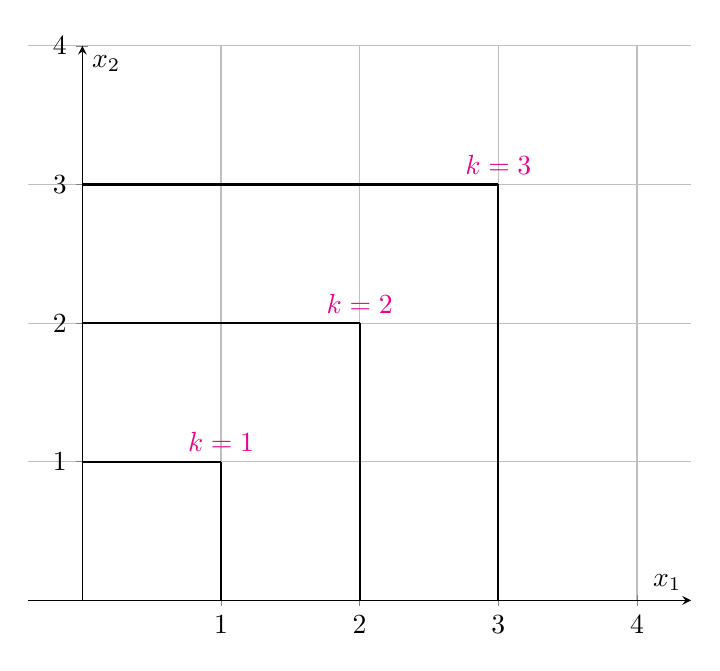
\begin{tikzpicture}[baseline]
           \begin{axis}[axis equal,
                        axis x line = middle,
                        axis y line = middle,
                        grid=both,
                        xmax=4,xmin=0,
                        ymin=0,ymax=4,
                        xlabel=$x_1$,ylabel=$x_2$,
                        xtick={0,...,4},
                        ytick={0,...,4},
                        width=10cm,
                        anchor=center]
             \addplot[thick] coordinates {(0,1)(1,1)};
             \addplot[thick] coordinates {(1,0)(1,1)};
             \draw (1, 1) node [magenta, above] {$k=1$};
             \addplot[thick] coordinates {(0,2)(2,2)};
             \addplot[thick] coordinates {(2,0)(2,2)};
             \draw (2, 2) node [magenta, above] {$k=2$};
             \addplot[thick] coordinates {(0,3)(3,3)};
             \addplot[thick] coordinates {(3,0)(3,3)};
             \draw (3, 3) node [magenta, above] {$k=3$};
           \end{axis}
         \end{tikzpicture}
       \end{center}
    }
  \item \textbf{[5 Points]} If $x_1=1$ and $x_2=2$, what is your $MRS$? Interpret the number.

    \textcolor{solution-color}{
      At $x_1=1$ and $x_2=2$, the slope of the indifference curve is 0 (it's
      flat). Therefore $MRS=0$ at that point. If we take away a small amount of
      $x_1$, you don't need to be compensated with any $x_2$ to stay on the
      same indifference curve since when $x_2<x_1$ it's only the amount of
      $x_2$ you have that matters for utility.
    }
  \item \textbf{[5 Points]} Find the demand functions $x_1\left( p_1,p_2,m \right)$ and $x_2\left(
    p_1,p_2, m\right)$

    \textcolor{solution-color}{
      It only matters which good we have the most of. If we bought a positive
      amount of both goods, the one with less will end up useless to us.
      Therefore we should only buy one good. Which one should we buy? The
      cheaper one! Therefore we have three cases like in the perfect
      substitute case: $p_1<p_2$, $p_1=p_2$ and $p_1>p_2$.
      \[
        x_1\left( p_1,p_2,m \right)=
        \begin{cases}
          \frac{m}{p_1} & \text{ if } p_1 < p_2 \\
          \text{Either } \frac{m}{p_1} \text{ or } 0 & \text{ if } p_1 = p_2 \\
          0 & \text{ if } p_1 > p_2 \\
        \end{cases}
      \]
      \[
        x_2\left( p_1,p_2,m \right)=
        \begin{cases}
          0 & \text{ if } p_1 < p_2 \\
          \text{Either } \frac{m}{p_2} \text{ or } 0 & \text{ if } p_1 = p_2 \\
          \frac{m}{p_2} & \text{ if } p_1 > p_2 \\
        \end{cases}
      \]
    }
  % \item Suppose initially $p_1>p_2$. Then $p_2$ increases so much that we end
  %   up with $p_2>p_1$. Does the demand for good 1 increase or decrease? Are the
  %   goods substitutes or complements?

    % \textcolor{solution-color}{
    %   If $p_1>p_2$, your demand for good 1 is zero (you spend all your money on
    %   good 2). If $p_2$ increases so much that good 1 becomes the cheaper good,
    %   you switch to only buying good 1. Thus your demand for good 1 increases.
    %   Since demand for good 1 and the price of good 2 are positively related,
    %   the goods are substitutes.
    % }
  % \item Can you come up with an example of two goods where you might have such
  %   preferences? Feel free to make assumptions about a particular scenario.

  %   \textcolor{solution-color}{
  %     From the demand function, we can see that the preferences are very close
  %     to perfect subtitutes. The only thing that is different is what you do
  %     when both prices are the same. With perfect substitutes you were
  %     indifferent between consuming all of one or the other or \emph{any
  %     combination of the two goods}. With these preferences you will still
  %     stick to one or the other when the price is the same and not mix and
  %     match.
  %   }

  %   \textcolor{solution-color}{
  %     You could make a simple extension to the old perfect substitutes example:
  %     red pencils and blue penciles. All you need to do is assume that it is
  %     illegal to have pencils that are different colors. If prices are
  %     different, you always buy the cheaper pencil. In the case where the
  %     prices are the same, you pick one color and stick with it.  You don't mix
  %     and match because it is illegal.
  %   }

  %   \textcolor{solution-color}{
  %     For a somewhat more realistic example, consider the following.
  %     Suppose there are two gaming consoles (e.g. PlayStation and Xbox). Both
  %     consoles have the exact same games on offer but you need to buy the game
  %     specific to the console. Suppose that otherwise the consoles are the same
  %     (same quality and cost the same). Assume further that it's before the
  %     internet so it didn't matter what console your friends have.
  %   }

  %   \textcolor{solution-color}{
  %     Good 1 here is games for PlayStation and good 2 is games for Xbox. You
  %     are trying to decide how many PlayStation games and Xbox games to buy.
  %     After you have bought the games you decide to buy one or both of the
  %     consoles. You decide that it doesn't make sense to buy games from both
  %     consoles because then you will need to buy both a PlayStation and an
  %     Xbox, which is expensive. So you only buy the games from one console. If
  %     you have the same game from two consoles, the extra game is useless to
  %     you.
  %   }
\end{subquestions}

\question{Income and Substitution Effects (10 Points)}
You live for one period. There are two goods with prices $p_1$ and $p_2$. You have income $m$ to spend on the two goods. Both goods are normal and your preferences satisfy all the main assumptions.

For each of the following parts, draw \textsl{\textbf{separate}} graphs.
\begin{subquestions}
\item \textbf{[2 Points]} Draw the budget line, your optimal consumption bundle and the indifference curve associated with the optimal choice. Label your axes and the points where the budget line intercepts the axes.
\begin{center}
  \begin{tikzpicture}[scale=0.9]
    \draw [thick] (0,0) -- (8,0);
    \draw [thick] (0,0) -- (0,5);
    \node [right] at (8,0) {$x_1$};
    \node [above] at (0,5) {$x_2$};
    \draw [thick] (0.6,4) to [out=295,in=165] (3.5,1);
    \draw [thick] (0,4.6) -- (3.15,0);
    \draw[dotted](1.4,2.5)--(1.4,0);
    \node [left] at (1.3,2.5) {$x^A$};
    \draw[fill] (1.4,2.5) circle [radius =0.06];
    \node [left] at (0,4.6) {$\frac{m}{p_2}$};
    \node [below] at (3.15,-0) {$\frac{m}{p_1}$};
  \end{tikzpicture}
\end{center}
\item \textbf{[3 Points]} The price of good 1 falls. Describe what happens in a diagram. Show your new budget line, optimal bundle and indifference curve associated with the optimal choice.
\begin{center}
  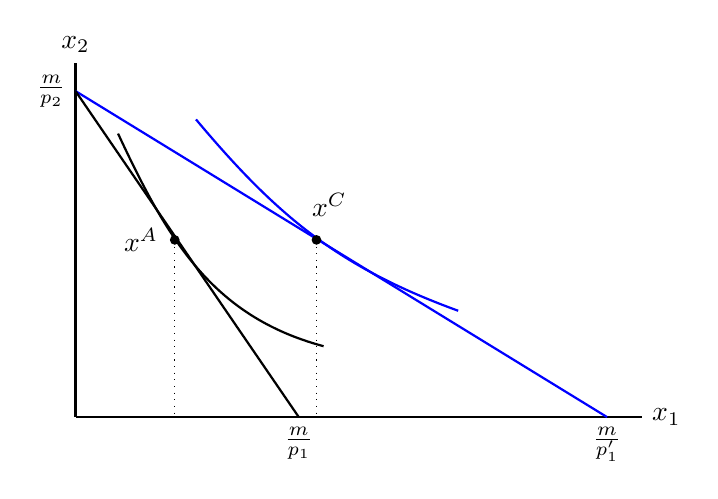
\begin{tikzpicture}[scale=0.9]
    \draw [thick] (0,0) -- (8,0);
    \draw [thick] (0,0) -- (0,5);
    \node [right] at (8,0) {$x_1$};
    \node [above] at (0,5) {$x_2$};
    \draw [thick, blue] (1.7,4.2) to [out=310,in=160] (5.4,1.5);
    \draw [thick] (0.6,4) to [out=295,in=165] (3.5,1);
    \draw [thick, blue] (0,4.6) -- (7.5,0);
    \draw [thick] (0,4.6) -- (3.15,0);
    \draw[dotted](1.4,2.5)--(1.4,0);
    \draw[dotted](3.4,2.5)--(3.4,0);
    \node [left] at (1.3,2.5) {$x^A$};
    \draw[fill] (1.4,2.5) circle [radius =0.06];
    \node [right] at (3.2,3) {$x^C$};
    \draw[fill] (3.4,2.5) circle [radius =0.06];
    \node [left] at (0,4.6) {$\frac{m}{p_2}$};
    \node [below] at (3.15,0) {$\frac{m}{p_1}$};
    \node [below] at (7.5,0) {$\frac{m}{p_1^\prime}$};
  \end{tikzpicture}
\end{center}
\item \textbf{[5 Points]} Decompose the change in demand for good 1 into income and substitution effects in a diagram. Show the optimal choice you would make if you only experienced a relative change in prices.
\begin{center}
  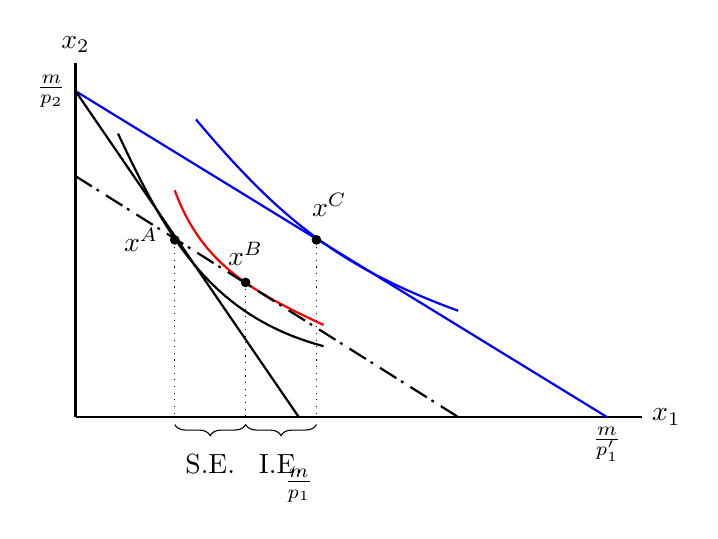
\begin{tikzpicture}[scale=0.9]
    \draw [thick] (0,0) -- (8,0);
    \draw [thick] (0,0) -- (0,5);
    \node [right] at (8,0) {$x_1$};
    \node [above] at (0,5) {$x_2$};
    \draw [thick, blue] (1.7,4.2) to [out=310,in=160] (5.4,1.5);
    \draw [thick] (0.6,4) to [out=295,in=165] (3.5,1);
    \draw [thick, red] (1.4,3.2) to [out=290,in=155] (3.5,1.3);
    \draw [thick, blue] (0,4.6) -- (7.5,0);
    \draw [thick] (0,4.6) -- (3.15,0);
    \draw[dotted](1.4,2.5)--(1.4,0);
    \draw[dotted](3.4,2.5)--(3.4,0);
    \draw [thick,dash pattern={on 7pt off 2pt on 1pt off 3pt}] (0,3.4) -- (5.4,0);
    \draw[dotted](2.4,1.9)--(2.4,0);
    \node [above] at (2.4,2) {$x^B$};
    \draw[fill] (2.4,1.9) circle [radius =0.06];
    \node [left] at (1.3,2.5) {$x^A$};
    \draw[fill] (1.4,2.5) circle [radius =0.06];
    \node [right] at (3.2,3) {$x^C$};
    \draw[fill] (3.4,2.5) circle [radius =0.06];
    \node [left] at (0,4.6) {$\frac{m}{p_2}$};
    \node [below] at (3.15,-0.6) {$\frac{m}{p_1}$};
    \node [below] at (7.5,0) {$\frac{m}{p_1^\prime}$};
    \draw [decorate,decoration={brace,amplitude=4pt, mirror},xshift=0pt,yshift=-3pt]
    (1.4,0) -- (2.4,0) node [black,midway,yshift=-.5cm] {S.E.};
    \draw [decorate,decoration={brace,amplitude=4pt, mirror},xshift=0pt,yshift=-3pt]
    (2.4,0) -- (3.4,0) node [black,midway,yshift=-.5cm] {I.E.};
  \end{tikzpicture}
\end{center}
\end{subquestions}

\question{Intertemporal Choice (5 Points)}
What is the most you would pay for a security that paid you \$100 in one year
from now and \$200 in two years from now? The interest rate is 5\%.

\textcolor{solution-color}{
  The security is worth:
  \[
    \frac{100}{1.05} + \frac{200}{\left(1.05\right)^2} = 95.2381 +
    181.4159=276.644
  \]
  Therefore you would pay up to \$276.64 for this security (if you can get
  it for less that's an even better deal).
}

\question{Uncertainty (15 Points)}
A Roulette wheel has 38 numbered pockets, labelled 0, 00, 1, 2, 3, \dots, 34, 35,
36. There are 18 red numbers, 18 black numbers and 2 green numbers (0 and 00).
The wheel is spun and a ball is thrown. The ball is equally likely to land on
any of the 38 pockets.

You have \$100. If you bet \$100 on red and it lands on red, you get \$200
back (your profit is \$100). If it lands on black or green, you get nothing
(you lose \$100).
\begin{subquestions}
  \item \textbf{[5 Points]} What is the expected value of wealth from taking the bet?

    \textcolor{solution-color}{
      The probability that you win is $\frac{18}{38}$. There are 38 possible
      pockets the ball can land in and 18 of them are red. The probability that
      you lose is $\frac{20}{38}$ (20 of the pockets are not red).
      The expected value of wealth is then:
      \[
        \frac{18}{38} \times \$200 + \frac{20}{38} \times \$0 = \$ 94.74
      \]
    }
  \item \textbf{[5 Points]} Suppose your utility function for wealth is $u\left( W
    \right)=\sqrt{W}$. Would you take this bet?

    \textcolor{solution-color}{
      Your expected utility from wealth from taking the bet is:
      \[
        \frac{18}{38} \times \sqrt{200} + \frac{20}{38} \times \sqrt{0} =
        6.6989
      \]
      If you don't take the bet you keep your \$100 and get expected utility
      $\sqrt{100}=10$. Since $10> 6.6989$ you shouldn't take the bet.
    }

  \item  \textbf{[5 Points]} Can you propose a utility function such that you would take this bet? Verify that indeed taking the bet with your proposed utility function is better than not taking it.

    \textcolor{solution-color}{
      Any convex utility function would work here since that would make you
      risk-loving. One simple example is $u\left( W \right)=W^2$. With this
      your expected utility is:
      \[
        \frac{18}{38} \times 200^2 + \frac{20}{38} \times 0^2 =
        18461.54
      \]
      If you don't take the bet your get expected utility $100^2=10000$ which
      is less than what you get from taking the bet.
    }
\end{subquestions}

\question{Technology (10 Points)}
Calculate (i) the marginal products of both factors of production and (ii) the
technical rate of substitution between both factors for the following
production function:
\[
  f\left( x_1,x_2 \right)=x_1^{\frac{1}{4}}x_2^{\frac{1}{2}}
\]
\textcolor{solution-color}{
  \[
    MP_1=\frac{\partial f\left( x_1,x_2 \right) }{\partial
    x_1}=\frac{1}{4}x_1^{\frac{1}{4}-1}x_2^{\frac{1}{2}}=
    \frac{1}{4}x_1^{-\frac{3}{4}}x_2^{\frac{1}{2}}
  \]
  \[
    MP_2=\frac{\partial f\left( x_1,x_2 \right) }{\partial
    x_2}=\frac{1}{2}x_1^{\frac{1}{4}}x_2^{\frac{1}{2}-1}=
    \frac{1}{2}x_1^{\frac{1}{4}}x_2^{-\frac{1}{2}}
  \]
  \[
    TRS=-\frac{MP_1}{MP_2}=
    -\frac{\frac{1}{4}x_1^{\frac{1}{4}-1}x_2^{\frac{1}{2}}}
    {\frac{1}{2}x_1^{\frac{1}{4}}x_2^{\frac{1}{2}-1}}=
    -\frac{1}{2}\frac{x_1^{-1}}{x_2^{-1}}=-\frac{1}{2}\frac{x_2}{x_1}
  \]
}

\question{Cost Curves (5 Points)}
The marginal cost function of a firm
is $MC\left( q \right)=2$. The firm has fixed costs of 5. What is the total cost
of producing $10$ units of output?

\textcolor{solution-color}{
  The variable cost of producing $q$ units of output is the sum of marginal
  costs up to $q$. Therefore the variable cost is $10\times2=20$. The fixed
  cost is 5 so the total cost is $20+5=25$.
}

\question{Firm Supply and Industry Supply (20 Points)}
All firms operating in a perfectly competitive industry have the same cost function $c\left( y\right) = y^2 +1$. The market demand function is $D\left( p \right)=100-10p$.
\begin{subquestions}
  \item \textbf{[3 Points]} What is each firm's supply function?

    \textcolor{solution-color}{
      The supply function expresses output in terms of price where $MC\left( y \right)=p$. Here $MC\left( y \right)=2y$ so setting $p=2y$ we can solve for output to get firm $i$'s supply function $S_i\left( p \right)=\frac{p}{2}$.
     }
  \item \textbf{[3 Points]} If there are 30 firms, what is the industry supply function?

    \textcolor{solution-color}{
      The industry supply function is the sum of the individual firms' supply functions:
      \[
        S\left( p \right)=\sum_{i=1}^{30} S_i\left( p \right)=30\times \frac{p}{2}=15p
      \]
     }
  \item \textbf{[3 Points]} If there are 30 firms, what is the equilibrium price?

    \textcolor{solution-color}{
      To get the equilibrium price, we set $S\left( p \right)=D\left( p \right)$ and solve for $p$:
      \begin{equation*}
        15p=100-10p \;\;\;\Longrightarrow\;\;\; 25p = 100 \;\;\;\Longrightarrow\;\;\; p=4
      \end{equation*}
     }
  \item \textbf{[3 Points]} If there are 30 firms, how much will each firm produce?

    \textcolor{solution-color}{
      We can just use $p=4$ in the individual firm's supply function $S\left( p \right)=\frac{p}{2}=\frac{4}{2}=2$.
     }
  \item \textbf{[3 Points]} If there are 30 firms, what is each firm's profits?

    \textcolor{solution-color}{
      Each firm will earn revenues of $p\times y= 4 \times 2 = 8$. The cost is $c\left( y \right)=y^2+1 = 2^2 + 1 = 4+1 = 5$. The profits are therefore $8-5=3$.
     }
  \item \textbf{[5 Points]} How many firms will there be in the long run?

    \textcolor{solution-color}{
      Since the firms are earning profits, other firms will enter in the long run. The task is to find out how many there will be. There are a number of ways you could answer this question.
    }\par\textcolor{solution-color}{
      \textbf{Method One:}
    }\par\textcolor{solution-color}{
      In the long run, firms make zero profits so price equals average cost. Since price equals marginal cost at the optimum, marginal cost equals average cost. So:
      \[
        MC\left( y \right)=AC\left( y \right) \;\;\;\Longrightarrow \;\;\;
        2y = \frac{y^2+1}{y} \;\;\; \Longrightarrow \;\;\;
        2y = y + \frac{1}{y} \;\;\; \Longrightarrow \;\;\;
        y=\frac{1}{y}\;\;\; \Longrightarrow \;\;\;
        y=1
    \]
    Each firm produces one unit in the long run. Since price equals average cost, we have $p=AC\left( y \right)=y+\frac{1}{y}=1+\frac{1}{1}=2$. The total demand will be $D\left( p \right)=100-10p=100-10\times 2 = 80$. If each firm produces 1 unit, then there will be $n=80$ firms in the long run.
    }\par\textcolor{solution-color}{
      \textbf{Method Two:}
    }\par\textcolor{solution-color}{
      Another way is to use the fact that industry supply and market demand will intersect at the minimum of average total cost. Average total cost here is $AC\left( y \right)=\frac{y^2+1}{y}=y+\frac{1}{y}$. Setting derivative of this equal to zero to find the minimum gives:
      \[1-\frac{1}{y^2}=0 \;\;\;\Longrightarrow \;\;\; y=1
      \]
      This says that in the long run each firm will produce 1 unit of output. At 1 unit of output  the average cost is $AC\left( 1 \right)=1+\frac{1}{1}=2$. Therefore the price must be 2 in the long run. At a price of 2, demand will be $100-10p=100-10\times 2 = 80$. Since supply equals demand in equilibrium, we will have that $n=80$. If each firm produces 1 unit, then there must be 80 firms to produce the 80 units to satisfy demand.
    }\par\textcolor{solution-color}{
      \textbf{Method Three:}
    }\par\textcolor{solution-color}{
      Another way to answer this is to use the fact that we know firms will earn zero profits in the long run. We can substitute the firm supply function $S_i\left( p \right)=\frac{p}{2}$ into the profit function:
      \begin{equation*}
        py - y^2 - 1 = p\left( \frac{p}{2} \right)-\left( \frac{p}{2} \right)^2 - 1=\frac{p^2}{2}-\frac{p^2}{4}-1=\frac{p^2}{4}-1
      \end{equation*}
      For profits to be zero we have $\frac{p^2}{4}-1=0$ so $p=2$. Using the firm supply function we find that $S_i\left( p \right)=\frac{p}{2}=\frac{2}{2}=1$. This is, each firm produces 1 unit of output. At a price of 2, industry supply will be $n\times\frac{p}{2}=n\times\frac{2}{2}=n$. At a price of 2, demand will be $100-10p=100-10\times 2 = 80$. Since supply equals demand in equilibrium, we will have that $n=80$. If each firm produces 1 unit, then there must be 80 firms to produce the 80 units to satisfy demand.
    }
\end{subquestions}

\question{Equilibrium and Taxation (15 Points)}
The demand and supply functions for good are:
\begin{align*}
  D\left( p \right) &= 120 - p \\
  S\left( p \right) &= 2p
\end{align*}
\begin{subquestions}
  \item \textbf{[5 Points]} Calculate the equilibrium price and quantity.

    \textcolor{solution-color}{
      To find the equilibrium price we set $D\left( p
      \right)=S\left( p \right)$:
      \[
         120-p^\star=2p^\star \;\;\;\Longleftrightarrow\;\;\;
         3p^\star=120 \;\;\;\Longleftrightarrow\;\;\;
         p^\star= \frac{120}{3}=40
      \]
      The equilibrium price is 40. To find the equilibrium quantity we can put
      this in either the demand function or the supply function (both will give
      the same answer). Using the supply function: $q^\star = 2p^\star = 2
      \times 40 = 80$. Therefore the equilibrium quantity is 80 units.
    }
\end{subquestions}
Suppose the government now adds a sales tax to the good of 20\%.
\begin{subquestions}
  \setcounter{enumi}{1}
  \item \textbf{[5 Points]} Calculate the price buyers pay, the price sellers receive and quantity
    sold after the tax is imposed.

    \textcolor{solution-color}{
      A sales tax means the price buyers pay is $\left( 1+\tau \right)$ times
      the price sellers receive, where $\tau$ is the tax rate. So $P_B=\left(
      1+\tau \right)P_S=1.2P_S$. The demand function then becomes:
      \[
        D\left( P_S \right)= 120 - 1.2 P_S
      \]
      To find the new equilibrium price, we set $D\left( P_S \right)=S\left(
      P_S \right)$:
      \[
        120-1.2 P_S = 2P_S \;\;\;\Longleftrightarrow\;\;\;
        3.2P_S=120 \;\;\;\Longleftrightarrow\;\;\;
        P_S=\frac{120}{3.2}=37.5
      \]
      The price the buyers pay is then:
      \[
        P_B = \left( 1+\tau \right)P_S = 1.2 \times 37.5 = 45
      \]
      The equilibrium quantity is then:
      \[
        q^\star = 2P_S = 2 \times 37.5 = 75.
      \]
      The price buyers pay increases from 40 to 45. The price sellers receive
      falls from 40 to 37.5. The quantity bought and sold falls from 80 to 75.
    }
  \item \textbf{[5 Points]} What portion of the tax to buyers pay and what portion of the tax do
    sellers pay?

    \textcolor{solution-color}{
      The total tax is 45-37.5=7.5. Of this, the buyers pay \$5 (difference
      between 45 and 40) and the sellers
      pay \$2.50 (difference between 40 and 37.5). Thus the portion the buyers
      pay is $\frac{2}{3}$ and the portion sellers pay $\frac{1}{3}$.
    }
\end{subquestions}
\end{document}
